\let\negmedspace\undefined
\let\negthickspace\undefined
%\RequirePackage{amsmath}
\documentclass[journal,12pt,twocolumn]{IEEEtran}
%
% \usepackage{setspace}
 \usepackage{gensymb}
%\doublespacing
 \usepackage{polynom}
%\singlespacing
%\usepackage{silence}
%Disable all warnings issued by latex starting with "You have..."
%\usepackage{graphicx}
\usepackage{amssymb}
%\usepackage{relsize}
\usepackage[cmex10]{amsmath}
%\usepackage{amsthm}
%\interdisplaylinepenalty=2500
%\savesymbol{iint}
%\usepackage{txfonts}
%\restoresymbol{TXF}{iint}
%\usepackage{wasysym}
\usepackage{amsthm}
%\usepackage{pifont}
%\usepackage{iithtlc}
% \usepackage{mathrsfs}
% \usepackage{txfonts}
 \usepackage{stfloats}
% \usepackage{steinmetz}
 \usepackage{bm}
% \usepackage{cite}
% \usepackage{cases}
% \usepackage{subfig}
%\usepackage{xtab}
\usepackage{longtable}
%\usepackage{multirow}
%\usepackage{algorithm}
%\usepackage{algpseudocode}
\usepackage{enumitem}
 \usepackage{mathtools}
 \usepackage{tikz}
% \usepackage{circuitikz}
% \usepackage{verbatim}
%\usepackage{tfrupee}
\usepackage[breaklinks=true]{hyperref}
%\usepackage{stmaryrd}
%\usepackage{tkz-euclide} % loads  TikZ and tkz-base
%\usetkzobj{all}
\usepackage{listings}
    \usepackage{color}                                            %%
    \usepackage{array}                                            %%
    \usepackage{longtable}                                        %%
    \usepackage{calc}                                             %%
    \usepackage{multirow}                                         %%
    \usepackage{hhline}                                           %%
    \usepackage{ifthen}                                           %%
  %optionally (for landscape tables embedded in another document): %%
    \usepackage{lscape}     
% \usepackage{multicol}
% \usepackage{chngcntr}
%\usepackage{enumerate}

%\usepackage{wasysym}
%\newcounter{MYtempeqncnt}
\DeclareMathOperator*{\Res}{Res}
\DeclareMathOperator*{\equals}{=}
%\renewcommand{\baselinestretch}{2}
\renewcommand\thesection{\arabic{section}}
\renewcommand\thesubsection{\thesection.\arabic{subsection}}
\renewcommand\thesubsubsection{\thesubsection.\arabic{subsubsection}}

\renewcommand\thesectiondis{\arabic{section}}
\renewcommand\thesubsectiondis{\thesectiondis.\arabic{subsection}}
\renewcommand\thesubsubsectiondis{\thesubsectiondis.\arabic{subsubsection}}

% correct bad hyphenation here
\hyphenation{op-tical net-works semi-conduc-tor}
\def\inputGnumericTable{}                                 %%

\lstset{
%language=C,
frame=single, 
breaklines=true,
columns=fullflexible
}
%\lstset{
%language=tex,
%frame=single, 
%breaklines=true
%}
\title{AI1110 ASSIGNMENT 1}
\author{Bandaru Naresh Kumar, AI21BTECH11006}
\begin{document}
\maketitle
\textbf{ICSE class 10 paper 2019}\\\\
\textbf{Q3 (b):}
M and N are two points on the X axis and Y axis respectively.
$P\left( 3,2\right)$ divides the line segment MN in the ratio 2:3.\\
Find:\\
 (i)the coordinates of M and N\\
 (ii)the slope of MN.\\\\
\\\textbf{Solution:}\\
Given,\\
\hspace*{10pt}M and N are two points on X and Y axes respectively.\\
\hspace*{10pt}Let M be $\left( a,0\right)$ and N be $\left( 0,b\right)$ \\
\hspace*{10pt}P divides MN in the ratio 2:3.\\
According to Section formula,\\\\
\hspace*{10pt}$P \equiv$ $\left(\dfrac{2(0)+3(a)}{2+3},\dfrac{2(b)+3(0)}{2+3}\right) $\\\\
\hspace*{10pt}$P \equiv$ $\left( \dfrac{3a}{5},\dfrac{2b}{5}\right) $\\\\
But we have,\\
\hspace*{10pt}$P \equiv$ (3,2)\\ 
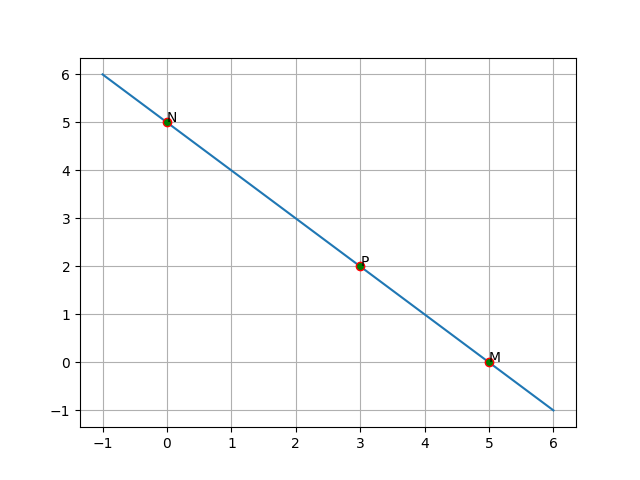
\includegraphics[scale=1]{figures/Figure_1.png}\\\\\\
Therefore,\\
\begin{align}
  &\dfrac{3a}{5} &= 3 \hspace{100pt} &\dfrac{2b}{5} &= 2 \\
 \implies &a &= 5 \hspace{100pt} &b &= 5
\end{align}\\ 
(i)$M \equiv$ (5,0) and $N \equiv$ (0,5)\\\\
(ii) Slope of MN = $\dfrac{5-0}{0-5}$\\\\
     \hspace*{85pt} = -1
\end{document}